Raviolimaskinen ska bestå av några mekaniska delar. För att designa maskinens delar ska CAD-tekniker användas. Att använda CAD-tekniker hjälper att rita maskinens olika delar och se resultatet innan man börjar konstruera dem fysiskt. Genom att designa med ett CAD-program, har man också möjligheten att analysera hållfasthet av maskinens delar genom att påverka virtuell kraft på dem. 


En mekanisk del av maskinen är en degform. Figuren ~\ref{degfrom} visar en dagform som används för att knyta Raviolidegen manuellt genom att trycka på formens sidor. För detta projekt har planerats att en eller två motorer ska trycka degformens sidor. Olika tekniker för att överföra motorers rörelseenergi till Raviolimaskinens degform ska undersökas. 

\begin{figure}[h]
	\begin{center}
		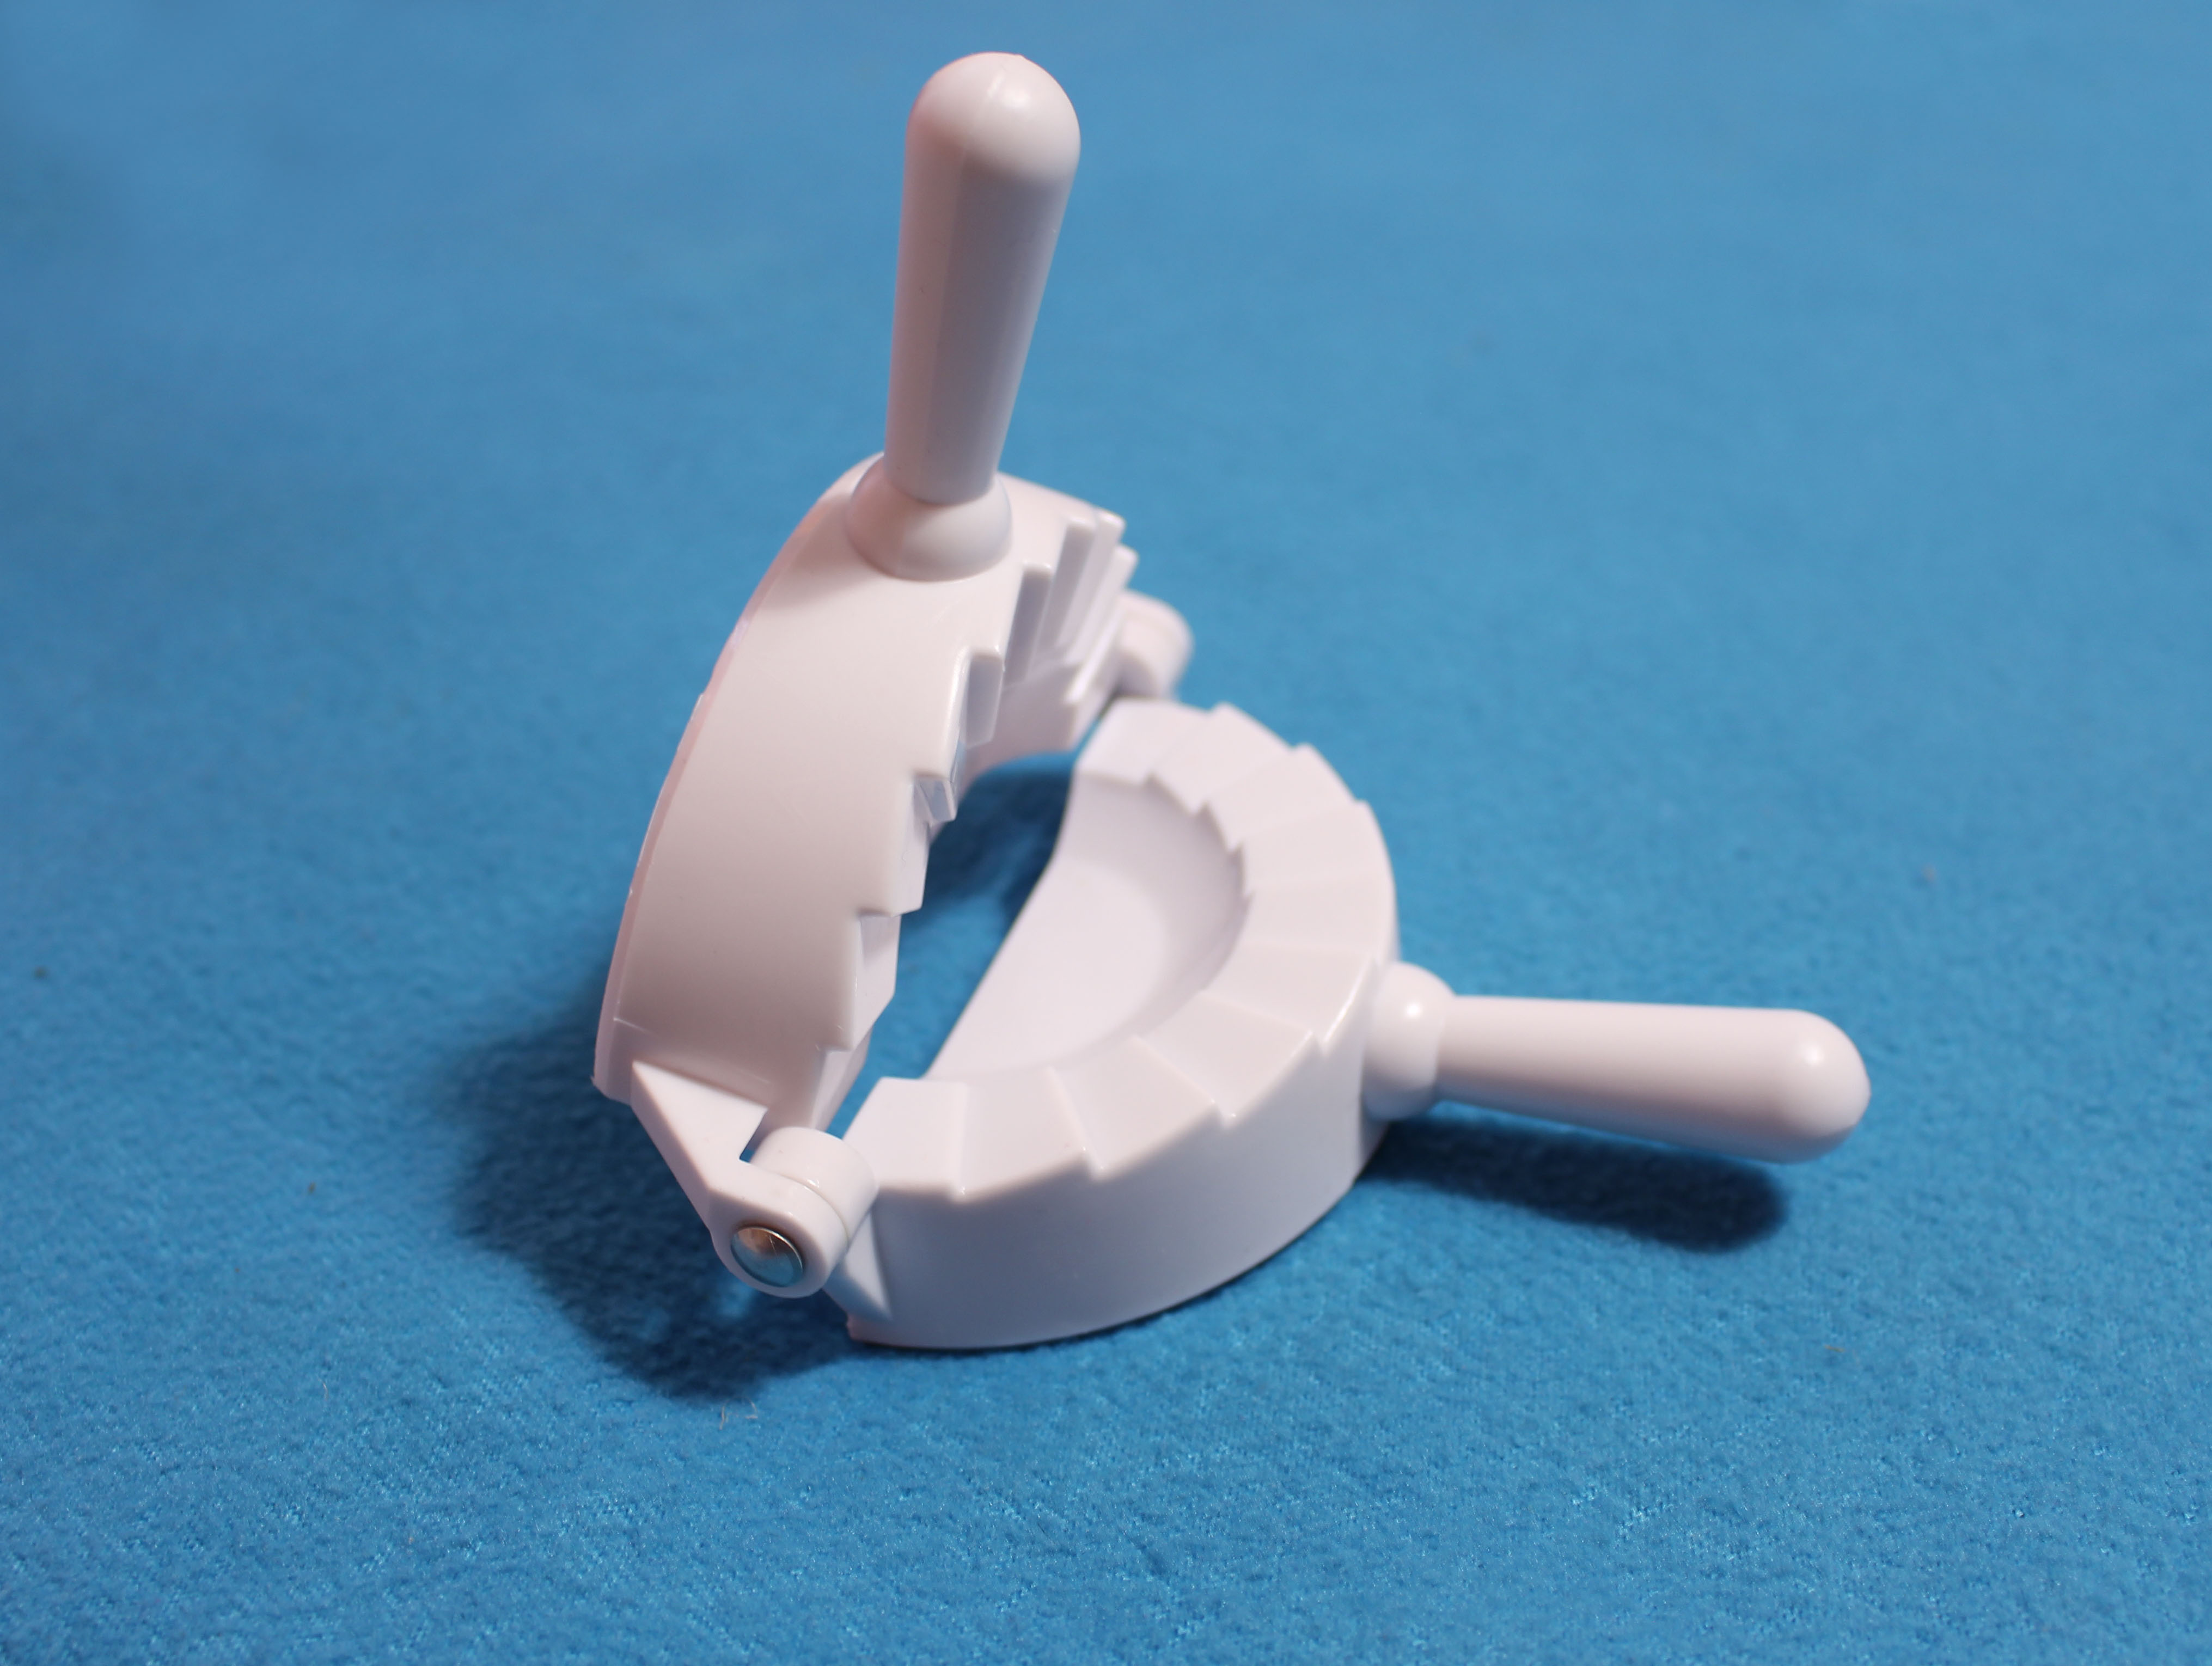
\includegraphics[scale=0.08] {images/degform.jpg}
		\caption{Degform för manuell ifyllning}
		\label{degfrom}	
	\end{center}
\end{figure}

En annan teknik som ska användas på detta projekt är regleringsteknik. Reglering kommer vara användbar när det gäller att reglera t.ex. den strömmen som går till elektroniska komponenter. Regleringsteknik kan också användas för eventuella systemidentifiering. 

Mikrokontrollern som ska användas för detta projekt är en Arduino Due. Programmeringsspråket ska vara C, men det är tänkt att använda Arduino IDE i fall man inte hinner programmera med C.




